%%%% Version 9 (2026-08-30). Short form of main_v8.tex for the IEEE Open Journal of
%%%% Engineering in Medicine and Biology (OJEMB), Technology Manuscript format.
%%%% No new experiments; every number is v8's, traced to the same artifacts:
%%%%   outputs/runs/modality_and_no_chewing_20260810T020642_cead62e4  (emg_only conditions)
%%%%   outputs/runs/baselines_emg_only_20260816                      (RQ3 architectures)
%%%%   outputs/screening/emg_only_filter_contrast.json                (RQ1 filter contrast)
%%%%   outputs/screening/emg_only_design.json                         (RQ4 design constraints)
%%%%   outputs/screening/emg_only_contrast.json                       (RQ3 feature baselines)
%%%%   outputs/data_audit/7ebbcc8d74c0bbe0/                           (guards, sweeps, mains)
%%%%   outputs/benchmarks/benchmark_emg_only.json                     (parameters, latencies)
%%%%
%%%% OJEMB limits applied (embs.org/ojemb/manuscript-formats, 2024/09 template):
%%%%   main body <= 3,000 words (references excluded), <= 8 display items, <= 50 references,
%%%%   structured abstract <= 150 words, impact statement <= 30 words, <= 5 index terms,
%%%%   conclusion <= 300 words, Visual Summary as page 1, Supplementary Materials in a
%%%%   separate document (main_v9_supp.tex) with <= 4,000 words and <= 10 display items.
%%%% Display items in this file: Figs. 1-4 and Tables I-IV (8). Everything else is in the
%%%% supplement and is referred to as Table S-I.. / Fig. S1.. from here.
%%%% Figures/v9/: fig1_system_pipeline.png (Paper/Picture1.png acquisition overview stacked over
%%%% Pipeline_V2.png, built by Figures/v9/make_fig1.py on 2026-09-07; it replaces the RL4 composite
%%%% fig1_pipeline_setup.png, whose cropped schematic left the electrode leads running off-panel),
%%%% fig3_errors.png (regenerated from the prediction ledger, same seed rule as Figures/v5),
%%%% visual_summary.pdf. refs_v8.bib entries were verified against Crossref on 2026-09-07.
\documentclass[journal]{IEEEtran}
\usepackage[usenames]{color}
\usepackage{xcolor}
\usepackage{epsfig}
\usepackage{graphics}
\usepackage{amsmath}
\usepackage{amssymb}
\usepackage{multirow}
\usepackage{cite}
\usepackage{array}
\usepackage{pslatex}
\usepackage{url}
\usepackage{caption}
\usepackage{graphicx}
\usepackage{setspace}
\usepackage{hhline}
\usepackage{mathtools}
\usepackage{booktabs}
\usepackage{textcomp}
\usepackage{pdfpages}
\usepackage[letterpaper]{geometry}
\geometry{verbose,tmargin=0.7in,bmargin=0.7in,lmargin=0.65in,rmargin=0.65in}
\setlength{\headheight}{17pt}
\setlength{\headsep}{5pt}
\newcommand{\flogo}{
\includegraphics[height=18pt]{embLogo.eps}}
\captionsetup[figure]{name={Fig.},labelsep=period,font=small}
\captionsetup[table]{name={TABLE},labelsep=period,font=small}
\usepackage[english]{babel}
\usepackage[utf8]{inputenc}
\usepackage{fancyhdr}
\pagestyle{fancy}
\fancyhf{}
\lhead{\flogo}
\rhead{\textcolor{violet}{\Large\textbf{Technology          }} \thepage}
\fancyfoot[CE,CO]{\leftmark}
\pagestyle{fancyplain}
\graphicspath{{./}{Figures/}}

\begin{document}

%%%% Page 1: Visual Summary (OJEMB requirement; drawn by make_visual_summary.py)
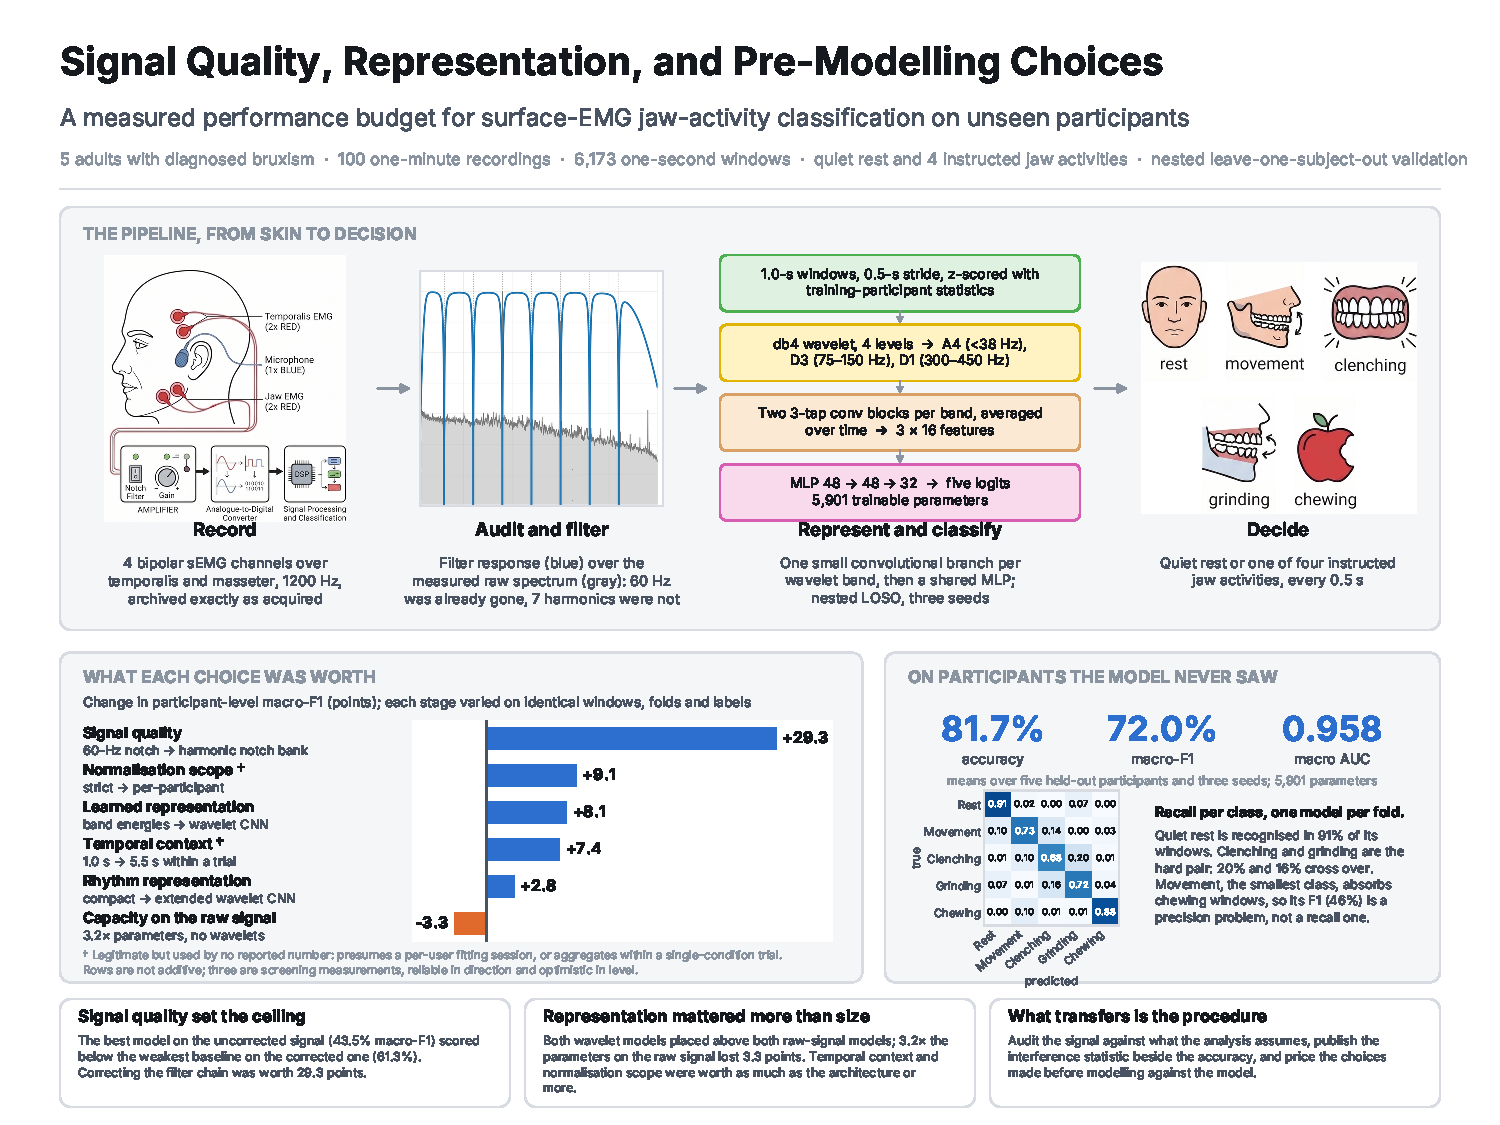
\includepdf[pages=1,pagecommand={\thispagestyle{empty}}]{Figures/v9/visual_summary.pdf}
\setcounter{page}{1}

\title{Signal Quality, Representation, and Pre-Modelling Choices: A Measured Performance Budget for Surface-EMG Jaw-Activity Classification on Unseen Participants}

\author{Mohammad~Hassan~Farhadi, Ali~Rabiee, Rahul~Singh, Mariusz~P.~Furmanek, Reza~Abiri*, and Theodore~A.~Walls*%
\thanks{Manuscript submitted September 7, 2026. This work was supported by an award from the Rhode Island Life Science Hub Small Grant Program (Principal Investigator T. A. Walls; Co-Investigators R. Abiri and M. P. Furmanek) and in part by the U.S. National Science Foundation under Grant 2245558 (Principal Investigator R. Abiri).}%
\thanks{M. H. Farhadi, A. Rabiee, R. Singh and R. Abiri are with the Department of Electrical, Computer, and Biomedical Engineering, University of Rhode Island, Kingston, RI, USA. M. P. Furmanek is with the Department of Physical Therapy, University of Rhode Island, Kingston, RI, USA, and with the Institute of Sport Sciences, Academy of Physical Education in Katowice, Katowice, Poland. T. A. Walls is with the Department of Psychology, University of Rhode Island, Kingston, RI, USA. *Corresponding authors: R. Abiri (e-mail: reza\_abiri@uri.edu) and T. A. Walls (e-mail: walls@uri.edu).}}

\markboth{Farhadi \MakeLowercase{\textit{et al.}}: A Measured Performance Budget for Surface-EMG Jaw-Activity Classification}{}

\maketitle\thispagestyle{fancy}

\begin{abstract}
\textit{Goal:} Pipelines that classify physiological signals are reported through a final accuracy that says little about which stage earned it. We ask which stages of one surface-electromyography (EMG) pipeline account for its performance. \textit{Methods:} One hundred recordings from five adults with diagnosed bruxism (quiet rest and four instructed jaw activities) were classified with a wavelet convolutional network under nested leave-one-subject-out validation. Each stage was then varied on identical windows, folds and labels, and its effect placed on one scale. \textit{Results:} Unseen-participant performance was 81.7\% accuracy and 72.0\% macro-F1. Correcting a mains-harmonic defect that a conventional single-notch chain had missed was worth 29.3 points of macro-F1; normalisation scope 9.1, learned representation 8.1, temporal context 7.4; tripling parameters on the raw signal lost 3.3. \textit{Conclusions:} Signal quality sets a ceiling, representation matters more than size, and choices fixed before modelling can outweigh the model. The procedure transfers to any biosignal pipeline.
\end{abstract}

\begin{IEEEkeywords}
Bruxism, convolutional neural networks, performance attribution, signal-quality audit, surface electromyography.
\end{IEEEkeywords}

\IEEEpeerreviewmaketitle

\textbf{\textit{Impact Statement---}Pricing each stage of an EMG classification pipeline on identical data showed signal quality, then representation, then pre-modelling choices outweighed model size: a procedure any biosignal study can apply.}\\

\section{Introduction}

\IEEEPARstart{A}{} classifier for physiological signals is the last stage of a long pipeline: a sensor, an amplifier with filters of its own, a filter chain, a segmentation rule, a normalisation scope and an evaluation protocol, any of which can move the reported number by more than the model. Yet pipelines in electromyography (EMG), electroencephalography (EEG), electrocardiography and inertial sensing are reported almost entirely through a final accuracy and a block diagram~\cite{thymi2021signal,roy2019deep}. Seed and split variance often exceeds the gains papers claim~\cite{bouthillier2021accounting}, and reporting standards now ask for an attribution a single accuracy cannot supply~\cite{kapoor2024reforms,collins2024tripod}.

This paper is a stage-by-stage analysis of one such pipeline. We built one pipeline end to end, from the participant's chair to the decision, and priced it: each stage is varied with everything else fixed, on the same windows, folds and labels, and the effects placed on one scale. Its parts, a signal audit, a wavelet decomposition, a small convolutional network and nested leave-one-subject-out (LOSO) evaluation, are deliberately standard, so that the budget measures the pipeline rather than a new model; what is new is that every stage reports what it was worth.

The case study is jaw activity from surface EMG. Bruxism, habitual clenching or grinding of the teeth, is common and hard to observe directly~\cite{lavigne2008bruxism,lavigne1996sleep}. Surface EMG records the jaw-closing muscles directly~\cite{raez2006techniques,colonna2023electromyographic}, but clenching, grinding and chewing all contract the same masseter and temporalis, and separating them on an unseen person is hard, yet good accuracies have been reported without an account of their origin~\cite{sonmezocak2021detection,gul2024advanced,ishtiaq2025wearable,heyat2020computational}. Prior studies (Supplementary Table~S-I) use small, mostly simulating cohorts and pooled validation, and vary only the classifier; we found none that reports a measured statement about the signal entering its pipeline, or that prices its segmentation and normalisation choices against its model. No public dataset supports such an analysis, so the data were collected for this study (Section~\ref{sec:data}).

Four questions are posed. \textbf{RQ1:} how much of what a classifier learns from these recordings is physiology, and how much is mains interference? \textbf{RQ2:} can four EMG channels separate quiet rest from four instructed jaw activities on an unseen participant? \textbf{RQ3:} which part of the model does the work: the wavelet representation, the architecture built on it, or the number of parameters? \textbf{RQ4:} how do those modelling choices compare with choices fixed before any model was trained: window length, temporal context and normalisation scope?

Signal quality sets a ceiling; below it, what a model can represent matters more than its size; and choices made before training were worth as much as the architecture or more. The contributions are the measured budget (Table~\ref{tab:budget}); the purpose-built dataset; a five-class result on unseen participants that includes quiet rest; a pipeline regenerated from a saved prediction ledger; and two inexpensive checks, drawing the filter response over the measured spectrum and fingerprinting every channel of every recording.

\section{Materials and Methods}

\subsection{Data}
\label{sec:data}

The study was approved by the Institutional Review Board of the University of Rhode Island (Protocol \#IRB22275690-2); every participant gave written informed consent, including consent to publish the identifying image in Fig.~\ref{fig:pipeline}(a). The recordings were collected for this study because no public dataset offers what the analysis needs: continuous recordings archived as acquired with a record of the hardware's own filtering, a synchronised marker, a quiet non-event condition, more than one food~\cite{zhang2018monitoring}, and raw files from which channel provenance can be verified (Supplementary Section~S-II).

\begin{figure*}[p]
  \centering
  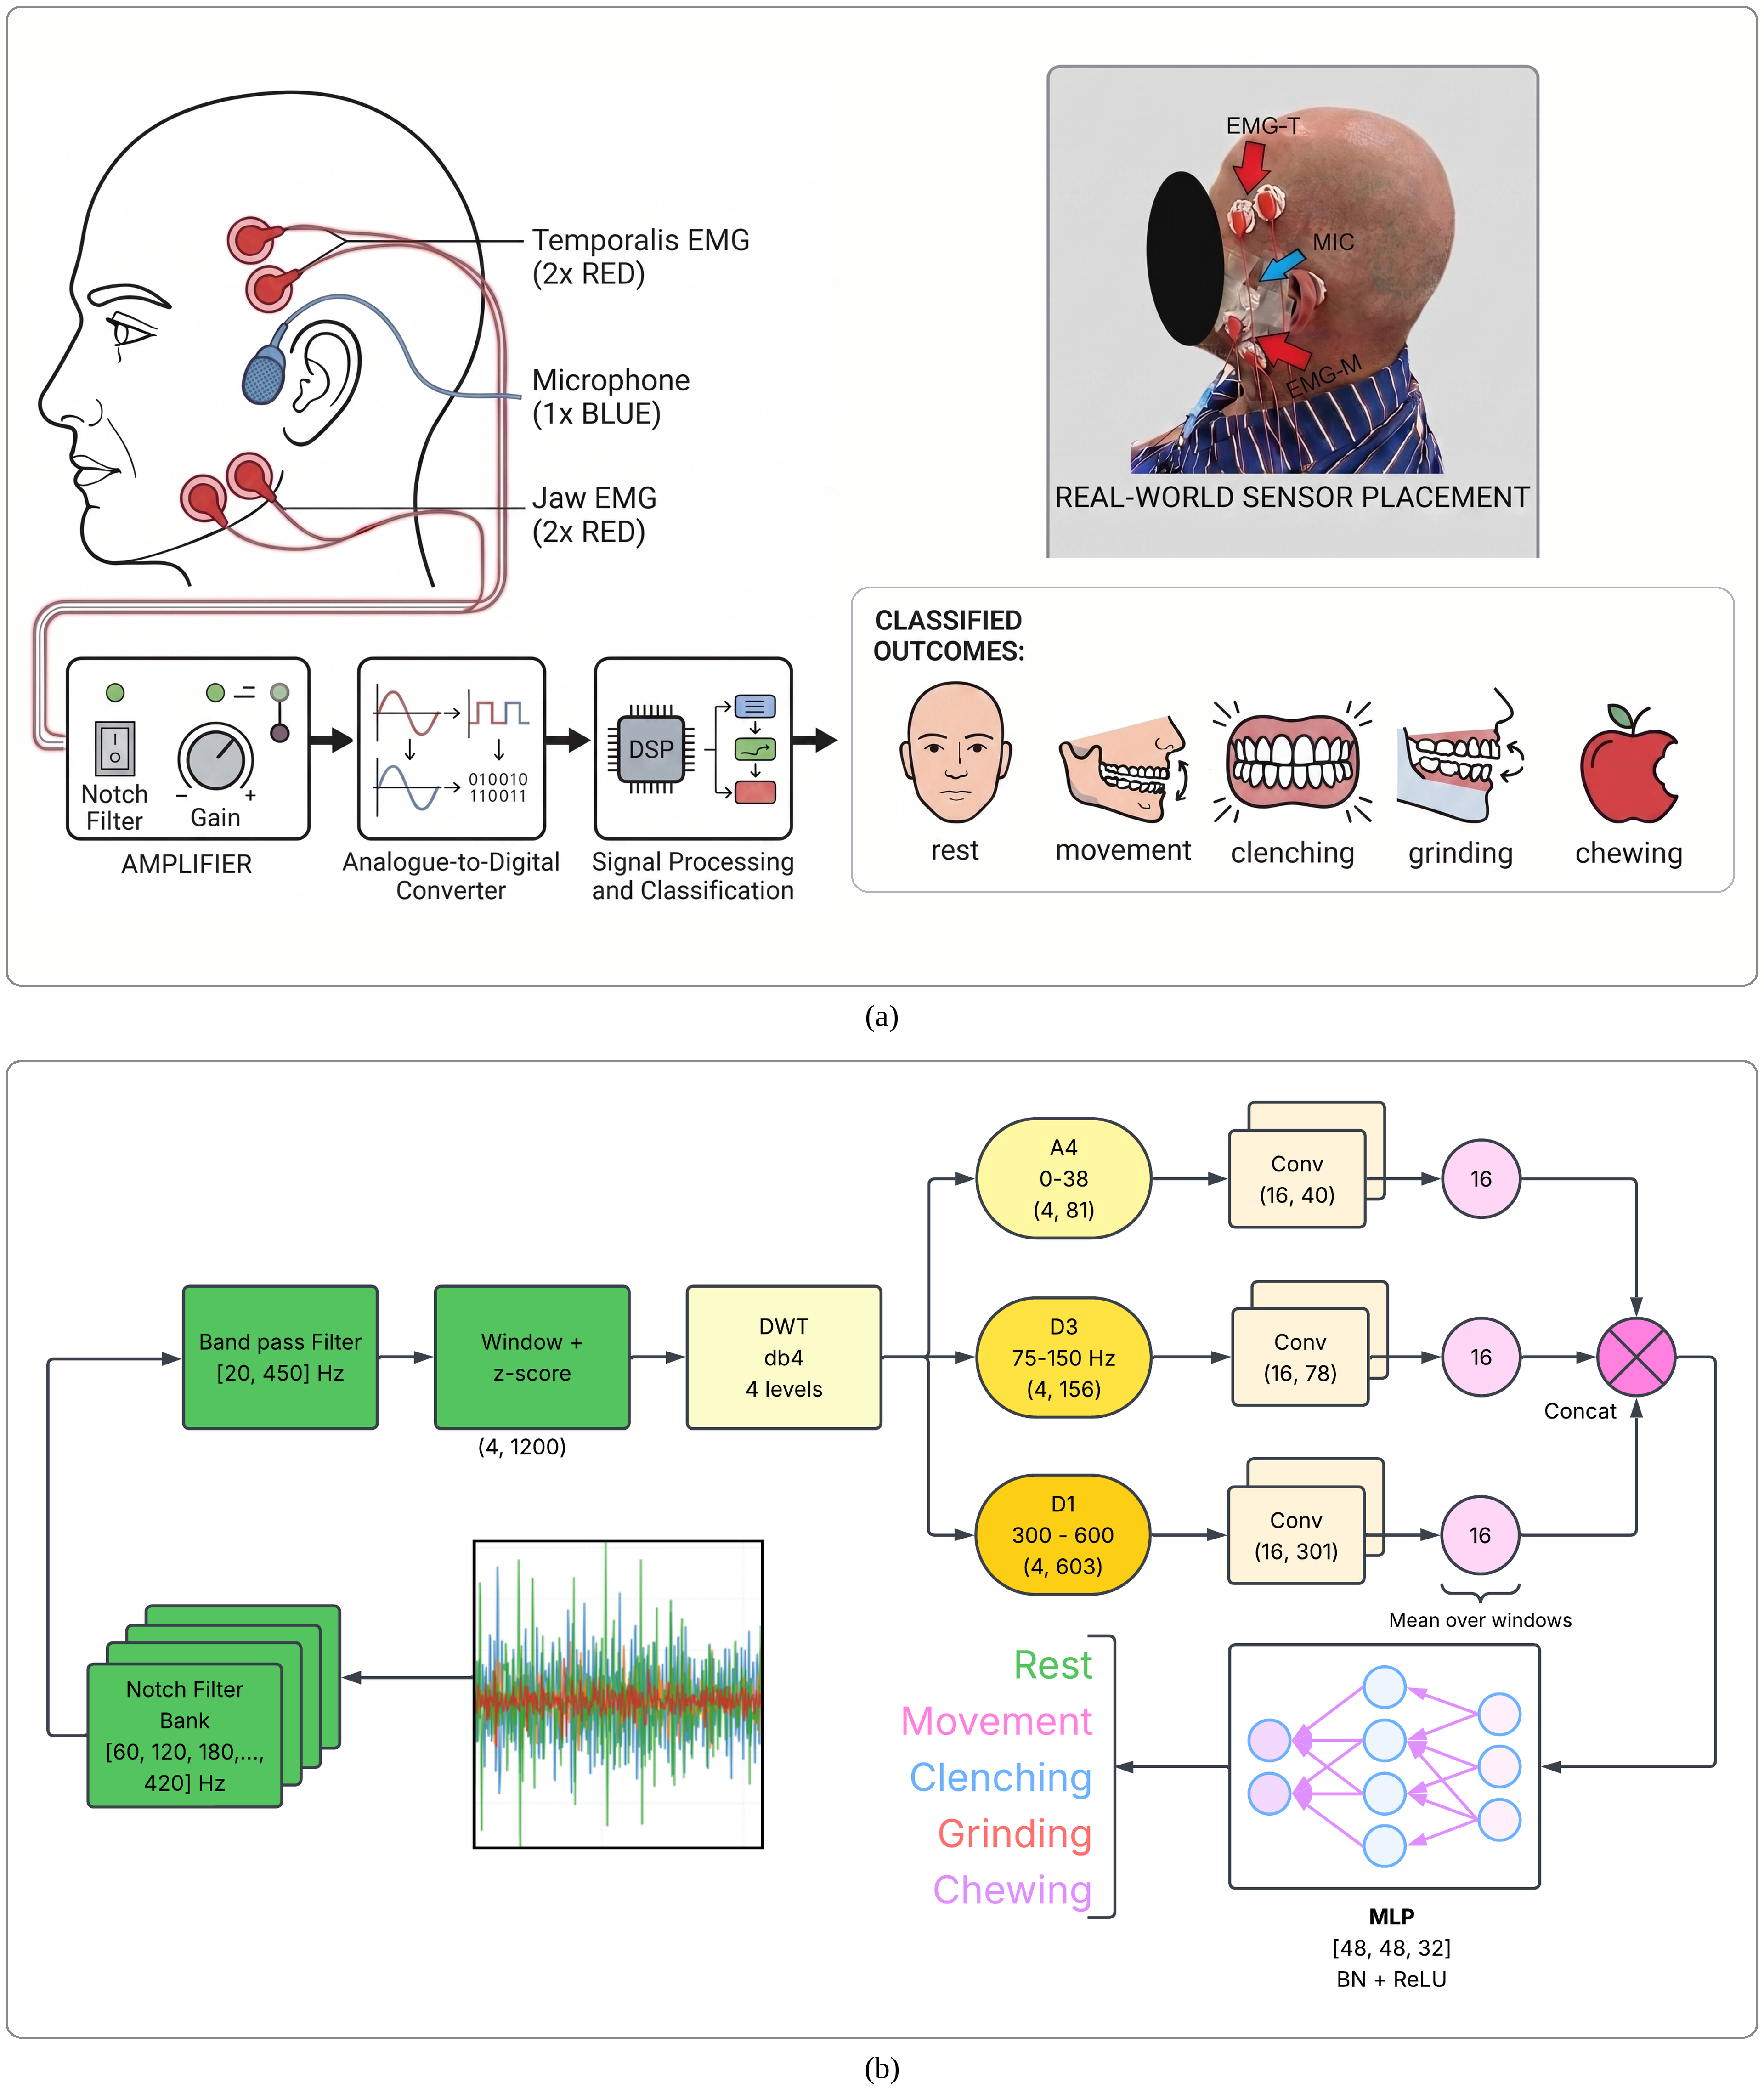
\includegraphics[width=0.97\textwidth]{Figures/v9/fig1_system_pipeline.png}
  \caption{System overview and reference model. (a) Acquisition chain: bipolar surface-EMG pairs over the temporalis and the masseter (``jaw'') on each side, four channels in all; the amplifier and acquisition software, whose own fixed notch is recorded in every metadata sidecar; the analogue-to-digital converter; and the processing that assigns each 1.0-s window to quiet rest or one of four instructed jaw activities. The microphone (blue) was recorded alongside and enters only the RQ1 contrast of Table~\ref{tab:filter}. Inset: placement on a participant (EMG-T, temporalis; EMG-M, masseter; MIC, microphone). (b) Reference model: the four channels pass through the notch bank and band-pass, are cut into 1.0-s windows, z-scored with training-participant statistics and decomposed with a four-level db4 transform; the retained bands $A_4$, $D_3$ and $D_1$ ($D_1$ occupies 300--450~Hz after the band-pass) each pass through two convolutional blocks and are averaged over the window's time axis to 16 features, and the 48 features enter an MLP ($48\rightarrow48\rightarrow32$) that produces five logits. The extended model of Table~\ref{tab:architectures} keeps the time axis instead of averaging it.}
  \label{fig:pipeline}
\end{figure*}

\subsection{Participants, Procedure and Sensors}

Five adults (two women, three men; age $38.0 \pm 10.4$ years) with a prior clinical diagnosis of bruxism performed every task on instruction, awake, in the laboratory: quiet rest; jaw movements (opening and closing, lateral deviation, protrusion and retrusion, biting); isometric molar and incisor clenching; instructed grinding; and chewing of cheese, carrots or popcorn, and gum, in twenty 1-min single-condition recordings per participant. A handheld button, pressed by the participant at task initiation, transmitted synchronised markers that are the sole source of the class labels. Four differential surface-EMG channels were recorded from bilateral bipolar pairs over the masseter and temporalis (Fig.~\ref{fig:pipeline}(a)); a camera served offline review, and a microphone, also recorded, enters only the RQ1 contrast (Table~\ref{tab:filter}). Signals were sampled at 1200~Hz and written to disk as acquired, with a metadata sidecar recording the acquisition software's own filter settings. Amplitudes are in arbitrary converter units, the hardware not being documented to current standards~\cite{isek1999standards,besomi2019consensus}.

\subsection{Windows and Labels}
\label{sec:windows}

Every analysed window lies wholly inside one marked task interval and is cut from the continuously filtered recording. Three measured exclusions apply (Supplementary Table~S-II): a 0.25-s guard at every marker edge and a 0.5-s startup guard, both sized from measured onset lags and settling transients, and quiet-rest windows drawn only from the five dedicated rest recordings. Five classes result: rest; movement; clenching (molar, incisor and unilateral bite); grinding; and chewing. Ninety-nine recordings yielded 6,173 analysable 1.0-s windows at a 0.5-s stride, 58.9\% of them chewing. The participant, not the window, is the unit of generalisation~\cite{saeb2017need}.

\subsection{Signal Validation and the Filter Chain}
\label{sec:filter}

The acquisition software applied its own fixed notch, recorded in every sidecar, which removed the 60-Hz fundamental before the data reached disk; interference survived at the harmonics, 180, 300 and 420~Hz, holding 91.3--99.8\% of the quiet-rest recordings' raw in-band power. The earlier chain (hereafter the superseded chain), a single 60-Hz notch ($Q=30$) followed by a 20--450-Hz band-pass, therefore removed a frequency that was already absent and passed every one that was present (Fig.~\ref{fig:filter}(a), (c)).

The corrected chain notches every mains multiple from 60 to 420~Hz before the same fourth-order Butterworth band-pass from 20 to 450~Hz~\cite{vanboxtel2001optimal,deluca2010filtering}. Each notch is 8~Hz wide at $-3$~dB rather than constant-$Q$: at an identical 13\% band cost the constant-width bank left eight times less residual interference, and the quiet-rest mains share fell to 0.46--0.66\% (Fig.~\ref{fig:filter}(b), (c)). The chain was selected on this criterion, not on held-out score (Supplementary Section~S-III). Harmonic notching is standard~\cite{mewett2004reducing,keshtkaran2014fast}; the novelty claimed is the check, not the remedy.

\begin{figure*}[!t]
  \centering
  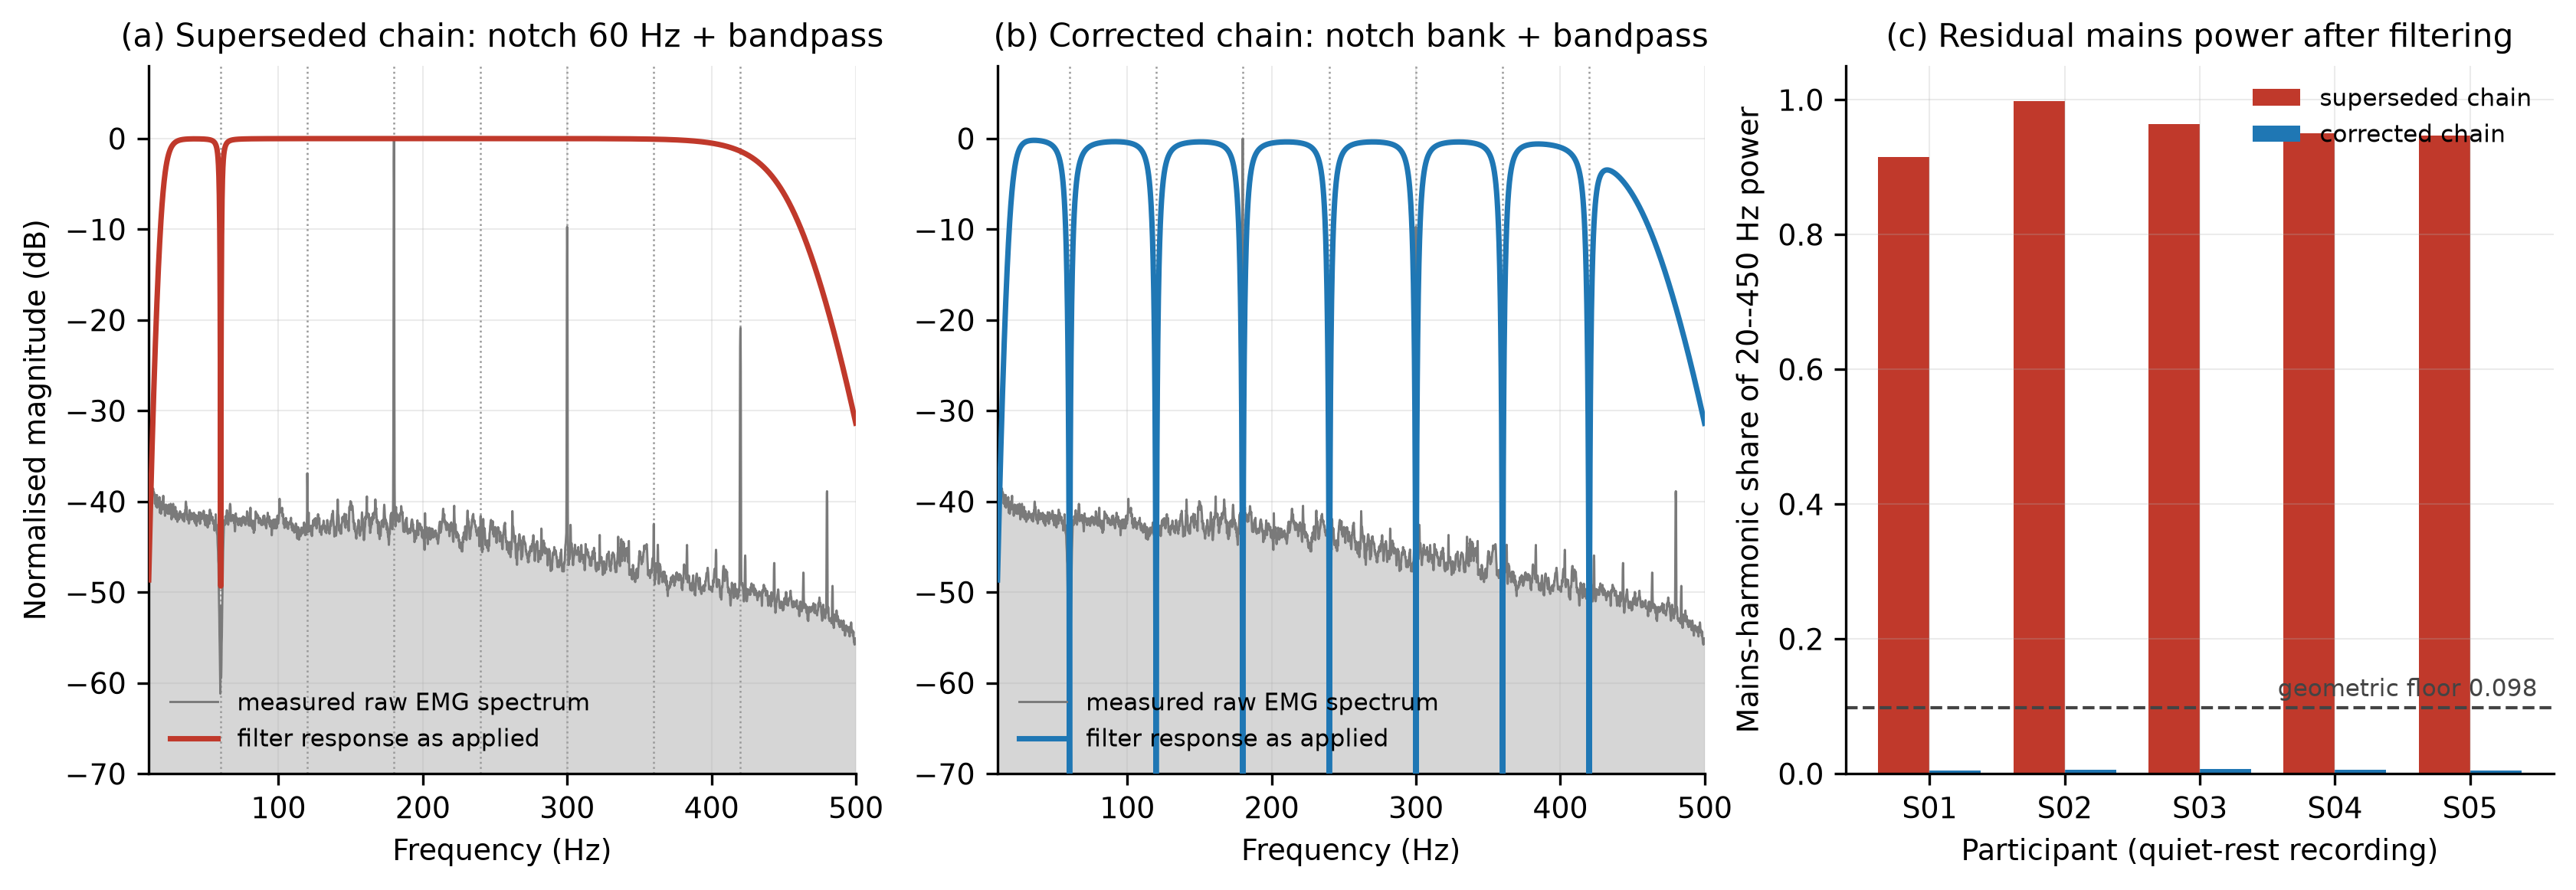
\includegraphics[width=0.94\textwidth]{Figures/filter_defect_and_correction.png}
  \caption{The mains-harmonic defect and its correction. (a) Superseded chain: the 60-Hz notch lands where the hardware had already removed the fundamental, while the harmonics at 180, 300 and 420~Hz pass untouched. (b) Corrected chain: seven constant-width notches land on the peaks. Gray traces are the mean raw spectrum of the five quiet-rest recordings, colored traces the response as applied, dotted lines the mains multiples. (c) Share of 20--450-Hz power within $\pm3$~Hz of a mains multiple, per participant, after each chain; the dashed line marks the 0.098 a white signal would score.}
  \label{fig:filter}
\end{figure*}

\subsection{Normalisation, Wavelet Decomposition and Model}

Channels were z-scored with statistics computed only from the training participants of the fold in question. Signals were decomposed with the Daubechies-4 wavelet at four levels~\cite{daubechies1992ten,englehart2003robust}, retaining $A_4$ (below 38~Hz), $D_3$ (75--150~Hz) and $D_1$ (300--450~Hz after the band-pass). The reference model (Fig.~\ref{fig:pipeline}(b)) gives each band two 3-tap convolutional blocks of 8 and 16 channels with batch normalisation and rectified linear units, averaged over the window's time axis to 16 features per band; the 48 features pass through a multilayer perceptron ($48\rightarrow48\rightarrow32$, dropout 0.5) to five logits, 5,901 trainable parameters in all.

\subsection{Training and Evaluation}
\label{sec:training}

Training used inverse-frequency class weights and minority-class augmentation, both confined to each fold's training partition, and AdamW~\cite{loshchilov2019decoupled} with focal loss~\cite{lin2017focal} in PyTorch~\cite{paszke2019pytorch}; the loss and learning rate were fixed rather than searched (Supplementary Table~S-II). Evaluation was nested LOSO~\cite{cawley2010overfitting,varma2006bias}: in each of five outer folds one participant was sealed as the test set, every statistic, weight, augmentation set and epoch budget was fitted inside a participant-grouped inner loop on the remaining four, and the held-out participant was scored exactly once; three seeds were run, none selected as best. Participant-level metrics, computed within each held-out participant and then averaged, are primary; pooled-window metrics are descriptive only, and no window-level intervals or $p$-values are reported, because the windows are clustered and $N=5$.

\subsection{Screening Harness and Safeguards}
\label{sec:screening}

A deliberately cheap screening harness supplies measurements the confirmatory protocol could not afford: 28 hand-crafted band-energy and waveform features per window~\cite{phinyomark2012feature}, with logistic regression and gradient boosting~\cite{pedregosa2011scikit} fitted once per outer fold. Because the features were chosen after seeing these participants, screening numbers are reliable in direction and optimistic in level. Three guards inside the pipeline refuse rather than warn: a leakage assertion on normalisation statistics, a check against wavelet bands the filter chain has removed, and a channel fingerprint against any held-out participant's signal appearing in its training set.

\section{Results}

The confirmatory results come from one nested-LOSO run on the corrected signal, 18,519 held-out predictions over five folds and three seeds, every value recomputed from the saved prediction ledger; pre-correction results appear only as RQ1's contrast arm.

\subsection{RQ1: How Much of the Signal Is Physiology}
\label{sec:rq1}

The filter chain was changed while the windows, folds and labels were held identical (Table~\ref{tab:filter}). Through the superseded chain the confirmatory network reached 55.0\% accuracy, 43.5\% participant-level macro-F1 and a macro AUC of 0.785; through the corrected chain the matched condition reached 80.9\%, 72.8\% and 0.963, a gain of 29.3 points of macro-F1, and the share of quiet-rest windows misread as clenching or grinding fell from 30.2\% to 6.1\%. The contrast is conservative: both arms are the EMG-plus-microphone condition, and the superseded arm additionally searched its loss and learning rate. The defect presented as between-participant heterogeneity: through the superseded chain P1 and P2 scored 18.1\% and 5.4\% macro-F1, at or below a constant prediction, whereas after correction all five participants span 61.4--82.4\%. A control chain with no mains removal scored within 1.2 points of the superseded chain, which was therefore inert (Supplementary Fig.~S2).

\begin{table*}[!t]
  \centering
  \caption{RQ1. Only the filter chain varies: the same 6,173 windows, fold assignments and labels in every arm. Residual mains is the share of 20--450-Hz power within $\pm3$~Hz of a mains multiple (a white signal scores 0.098); ``Inv.'' counts participant pairs in which one person's resting EMG exceeded another's active EMG.}
  \label{tab:filter}
  \footnotesize
  \begin{tabular*}{\textwidth}{@{\extracolsep{\fill}}lcccccc@{}}
    \toprule
    & \multicolumn{3}{c}{Measured signal properties} & \multicolumn{3}{c}{Participant-level macro-F1} \\
    \cmidrule(lr){2-4}\cmidrule(lr){5-7}
    EMG chain & Residual mains & Ampl.\ spread & Inv. & Wavelet CNN$^{a}$ & Logistic reg.$^{b}$ & Grad.\ boost.$^{b}$ \\
    \midrule
    60-Hz notch only (superseded) & 0.673 & $5.07\times$ & 20 & 43.5\% & 37.3\% & 38.8\% \\
    Band-pass only (control) & 0.671 & $5.02\times$ & 20 & --- & 38.5\% & 39.2\% \\
    \textbf{Mains notch bank, 8 Hz (used)} & \textbf{0.012} & $\mathbf{2.97\times}$ & \textbf{0} & \textbf{72.8\%} & \textbf{63.9\%} & \textbf{61.3\%} \\
    \bottomrule
  \end{tabular*}
  \begin{flushleft}\footnotesize
  $^{a}$Confirmatory nested LOSO, three seeds; both rows the EMG-plus-microphone condition, the superseded row additionally searching loss and learning rate, so the comparison favours the superseded arm. The corrected EMG-only condition scores 72.0\%.
  $^{b}$Screening harness, one fit per outer fold, no nested selection; optimistic in level.
  \end{flushleft}
\end{table*}

\subsection{RQ2: Five Classes on Unseen Participants}
\label{sec:rq2}

Averaged over the five held-out participants and three seeds, the reference model achieved 81.7\% accuracy, 72.0\% macro-F1 and a macro ROC--AUC of 0.958 (Table~\ref{tab:results}). Quiet rest reached 77.1\% precision, 91.4\% recall and an F1 of 83.6\%, the best-recalled class. Movement's F1 of 46.0\% is a precision problem (Fig.~\ref{fig:errors}), 34.4\% precision at 69.8\% recall, because the smallest class absorbs 9.9\% of the eleven-times-more-numerous chewing windows~\cite{saito2015precision}. Clenching and grinding are the hardest pair, 19.5\% of clenching windows labelled grinding and 14.5\% of grinding windows clenching. Rest's dominant error was into grinding, 7.5\%, so 7.7\% of quiet-rest windows fell on the tooth-contact side, the closest analogue of a false-alarm rate available here. Secondary analyses are in Supplementary Table~S-III, ROC curves and a t-SNE in Supplementary Fig.~S3.

\begin{table*}[!t]
  \centering
  \caption{Five-class performance on the corrected signal: participant-level means over five held-out participants and three seeds (upper block); per-class values on pooled held-out windows, averaged over seeds (middle); and each held-out participant, averaged over seeds (lower). Values describe this five-participant dataset and are not population-level tests.}
  \label{tab:results}
  \footnotesize
  \begin{tabular*}{\textwidth}{@{\extracolsep{\fill}}lcccccc@{}}
    \toprule
    Method / class / participant & Accuracy & Precision & Recall & F1 & AUC & Windows \\
    \midrule
    \multicolumn{7}{l}{\emph{Participant-level means, five held-out participants $\times$ three seeds}}\\
    \textbf{Wavelet CNN, 4-channel EMG} & \textbf{81.7\%} & \textbf{73.7\%} & \textbf{77.6\%} & \textbf{72.0\%} & \textbf{0.958} & 6,173 \\
    Logistic regression, band energies$^{a}$ & 78.3\% & --- & --- & 63.9\% & 0.965 & 6,173 \\
    Gradient boosting, band energies$^{a}$ & 74.8\% & --- & --- & 61.3\% & 0.914 & 6,173 \\
    \midrule
    \multicolumn{7}{l}{\emph{Wavelet CNN, per class, pooled held-out windows}}\\
    Rest & --- & 77.1\% & 91.4\% & 83.6\% & 0.958 & 590 \\
    Movement & --- & 34.4\% & 69.8\% & 46.0\% & 0.937 & 333 \\
    Clenching & --- & 70.5\% & 66.0\% & 68.1\% & 0.936 & 799 \\
    Grinding & --- & 67.9\% & 69.5\% & 68.6\% & 0.928 & 816 \\
    Chewing & --- & 97.3\% & 85.8\% & 91.1\% & 0.981 & 3,635 \\
    Macro average & 80.7\% & 69.4\% & 76.5\% & 71.5\% & 0.948 & 6,173 \\
    \midrule
    \multicolumn{7}{l}{\emph{Wavelet CNN, per held-out participant, three-seed means}}\\
    Participant 1 & 73.4\% & --- & --- & 63.2\% & 0.904 & 1,692 \\
    Participant 2 & 90.7\% & --- & --- & 72.6\% & 0.957 & 1,007 \\
    Participant 3 & 83.7\% & --- & --- & 71.3\% & 0.967 & 1,133 \\
    Participant 4 & 74.0\% & --- & --- & 72.2\% & 0.981 & 1,167 \\
    Participant 5 & 86.7\% & --- & --- & 80.5\% & 0.980 & 1,174 \\
    Standard deviation across participants & 7.7 & --- & --- & 6.1 & 0.032 & --- \\
    \bottomrule
  \end{tabular*}
  \begin{flushleft}\footnotesize
  $^{a}$Screening harness (Section~\ref{sec:screening}), optimistic in level, which makes the network's margin conservative; the harness stores no per-class table.
  \end{flushleft}
\end{table*}

\begin{figure*}[!t]
  \centering
  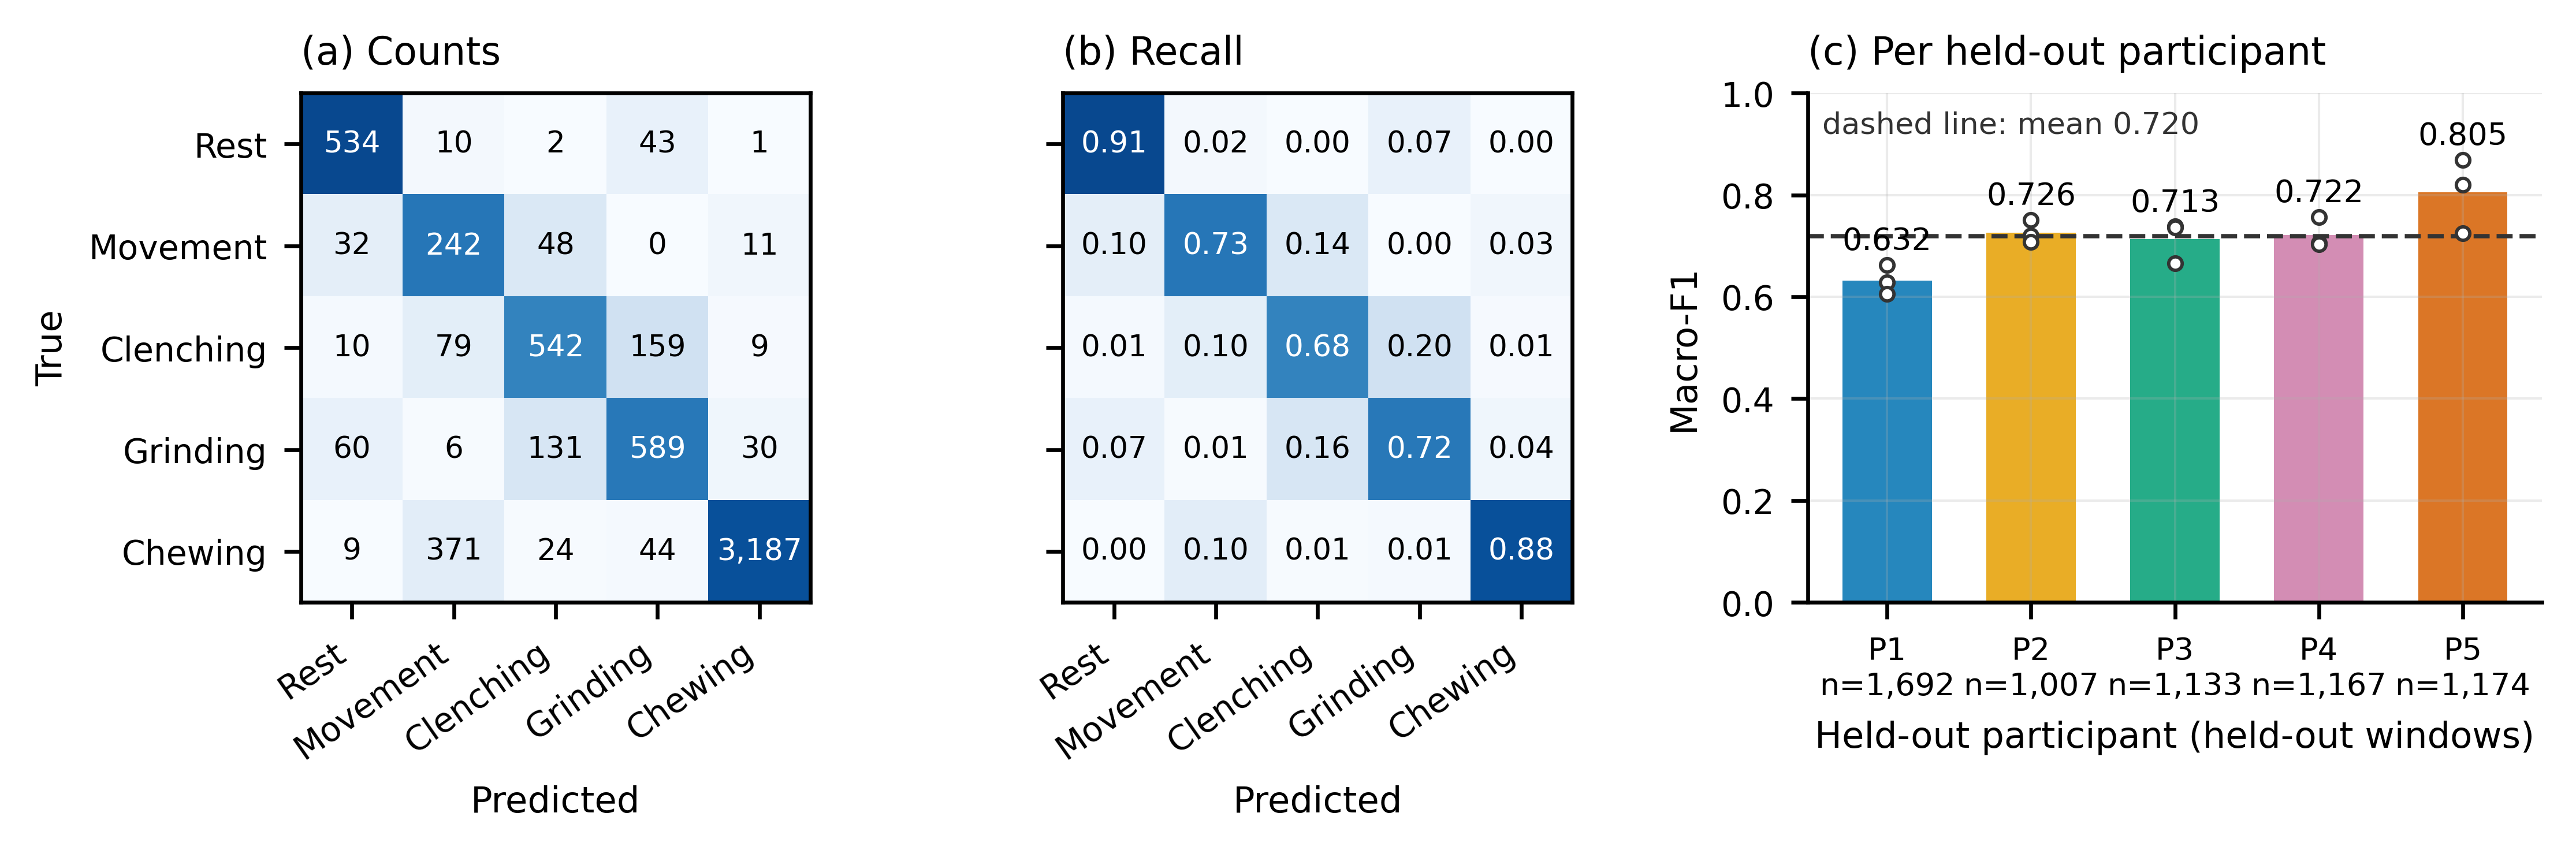
\includegraphics[width=0.98\textwidth]{Figures/v9/fig3_errors.png}
  \caption{Held-out behaviour of the reference model. (a) Confusion counts and (b) row-normalised recall, pooled across the five LOSO folds of seed 0, chosen by the fixed rule of lowest seed index. (c) Macro-F1 per held-out participant: bars are means over three seeds, open markers the individual seeds, and the label inside each bar that participant's held-out window count.}
  \label{fig:errors}
\end{figure*}

\subsection{RQ3: Representation, Architecture and Capacity}
\label{sec:rq3}

Logistic regression on the 28 screening features reached 63.9\% macro-F1 and gradient boosting 61.3\% (Table~\ref{tab:results}); the network's 72.0\% exceeds them by 8.1 and 10.6 points, a conservative margin given the harness's optimism. The two rank windows about equally well (macro AUC 0.965 against 0.958), so the network's advantage lies in where its decision boundaries fall; before the filter correction it had been only about four points, because when interference dominates a window a pooled band amplitude is all there is to extract (Supplementary Section~S-IV).

A prespecified sweep then contrasts four architectures under one training configuration on identical inputs (Table~\ref{tab:architectures}): the compact reference model; an extended member of the same family that keeps the time axis and adds a modulation-spectrum head, making 1--2-Hz rhythm representable within a window; and an early-fusion CNN and a bidirectional LSTM that read the raw channels without the wavelet decomposition. The grouping is the result: both wavelet models place above both raw-signal models, and the ordering does not follow parameter count, the early-fusion CNN reaching 68.9\% macro-F1 with 3.2 times the compact model's parameters against its 72.2\%, and the LSTM 60.2\%. Within the wavelet family the extended model is stronger, 75.0\% macro-F1 and 0.974 AUC against 72.2\% and 0.954, consistently across seeds but on three of the five participants, at three times the parameters and 2.2 times the latency. The compact model remains the reference: a 2.8-point difference resting on three of five participants is a direction rather than an effect size, it delivers 96\% of the extended model's macro-F1 at 33\% of the parameters, and the two are one family, so the extended model's advantage supports the representational argument.

\begin{table*}[!t]
  \centering
  \caption{RQ3. Four architectures on identical inputs, windows, folds and seeds under one training configuration, grouped by front end. Participant-level means $\pm$ standard deviation across seeds; ``Forward'' is the median forward pass for one window at batch size 1 on an Intel CPU.}
  \label{tab:architectures}
  \footnotesize
  \begin{tabular*}{\textwidth}{@{\extracolsep{\fill}}lrrcccc@{}}
    \toprule
    Architecture & Params & Forward & Accuracy & Bal.\ acc. & Macro-F1 & Macro AUC \\
    \midrule
    \multicolumn{7}{l}{\emph{db4 wavelet front end}}\\
    Wavelet CNN, extended$^{a}$ & 17,981 & 2.21 ms & $\mathbf{86.1 \pm 1.1}$\% & $\mathbf{78.9 \pm 0.9}$\% & $\mathbf{75.0 \pm 1.3}$\% & $\mathbf{0.974 \pm 0.003}$ \\
    Wavelet CNN, compact (reference)$^{b}$ & 5,901 & 1.02 ms & $81.0 \pm 2.2$\% & $77.4 \pm 1.0$\% & $72.2 \pm 1.5$\% & $0.954 \pm 0.006$ \\
    \midrule
    \multicolumn{7}{l}{\emph{No wavelet decomposition}}\\
    Early-fusion CNN, raw signals & 19,029 & 0.20 ms & $79.0 \pm 0.8$\% & $74.3 \pm 1.3$\% & $68.9 \pm 1.5$\% & $0.949 \pm 0.004$ \\
    Bidirectional LSTM & 10,053 & 1.16 ms & $71.5 \pm 3.3$\% & $66.4 \pm 2.5$\% & $60.2 \pm 2.6$\% & $0.898 \pm 0.013$ \\
    \bottomrule
  \end{tabular*}
  \begin{flushleft}\footnotesize
  $^{a}$The reference model with the time axis kept, plus mean, standard-deviation and maximum pooling per band and a modulation-spectrum head; its advantage rests on three of the five participants.
  $^{b}$The sweep's own measurement of the reference model; the confirmatory run reached 72.0\% (Table~\ref{tab:results}) on a different code revision.
  \end{flushleft}
\end{table*}

\subsection{RQ4: Three Choices Fixed Before Modelling}
\label{sec:rq4}

Three design choices were priced with the screening harness (Fig.~\ref{fig:design}); two are worth as much as the 8.1-point architectural margin or more. First, the 1.0-s window is a binding constraint, not a tuned parameter: chewing and grinding differ from clenching partly by 1--2-Hz rhythm (Supplementary Fig.~S4), and aggregating held-out probabilities over consecutive windows raises macro-F1 monotonically from 0.730 at 1.0~s to 0.804 at 5.5~s. Because every recording holds one condition, that 7.4-point gain is a trial-level estimate, not a streaming result. Second, because participants marked intervals at very different granularity, the guard sweep alone moves the smallest participant-and-class cell from 50 windows to 1; the resolution is to standardise trigger use at collection. Third, normalisation scope is worth about as much as the architecture: standardising each participant's features by that participant's own unlabelled distribution raises the screening classifier from 0.639 to 0.730 macro-F1, transductive adaptation that is legitimate but presumes a per-user fitting session, so it is used by no reported number. Training curves and latencies are in Supplementary Fig.~S5; no real-time claim is made.

\begin{figure*}[!t]
  \centering
  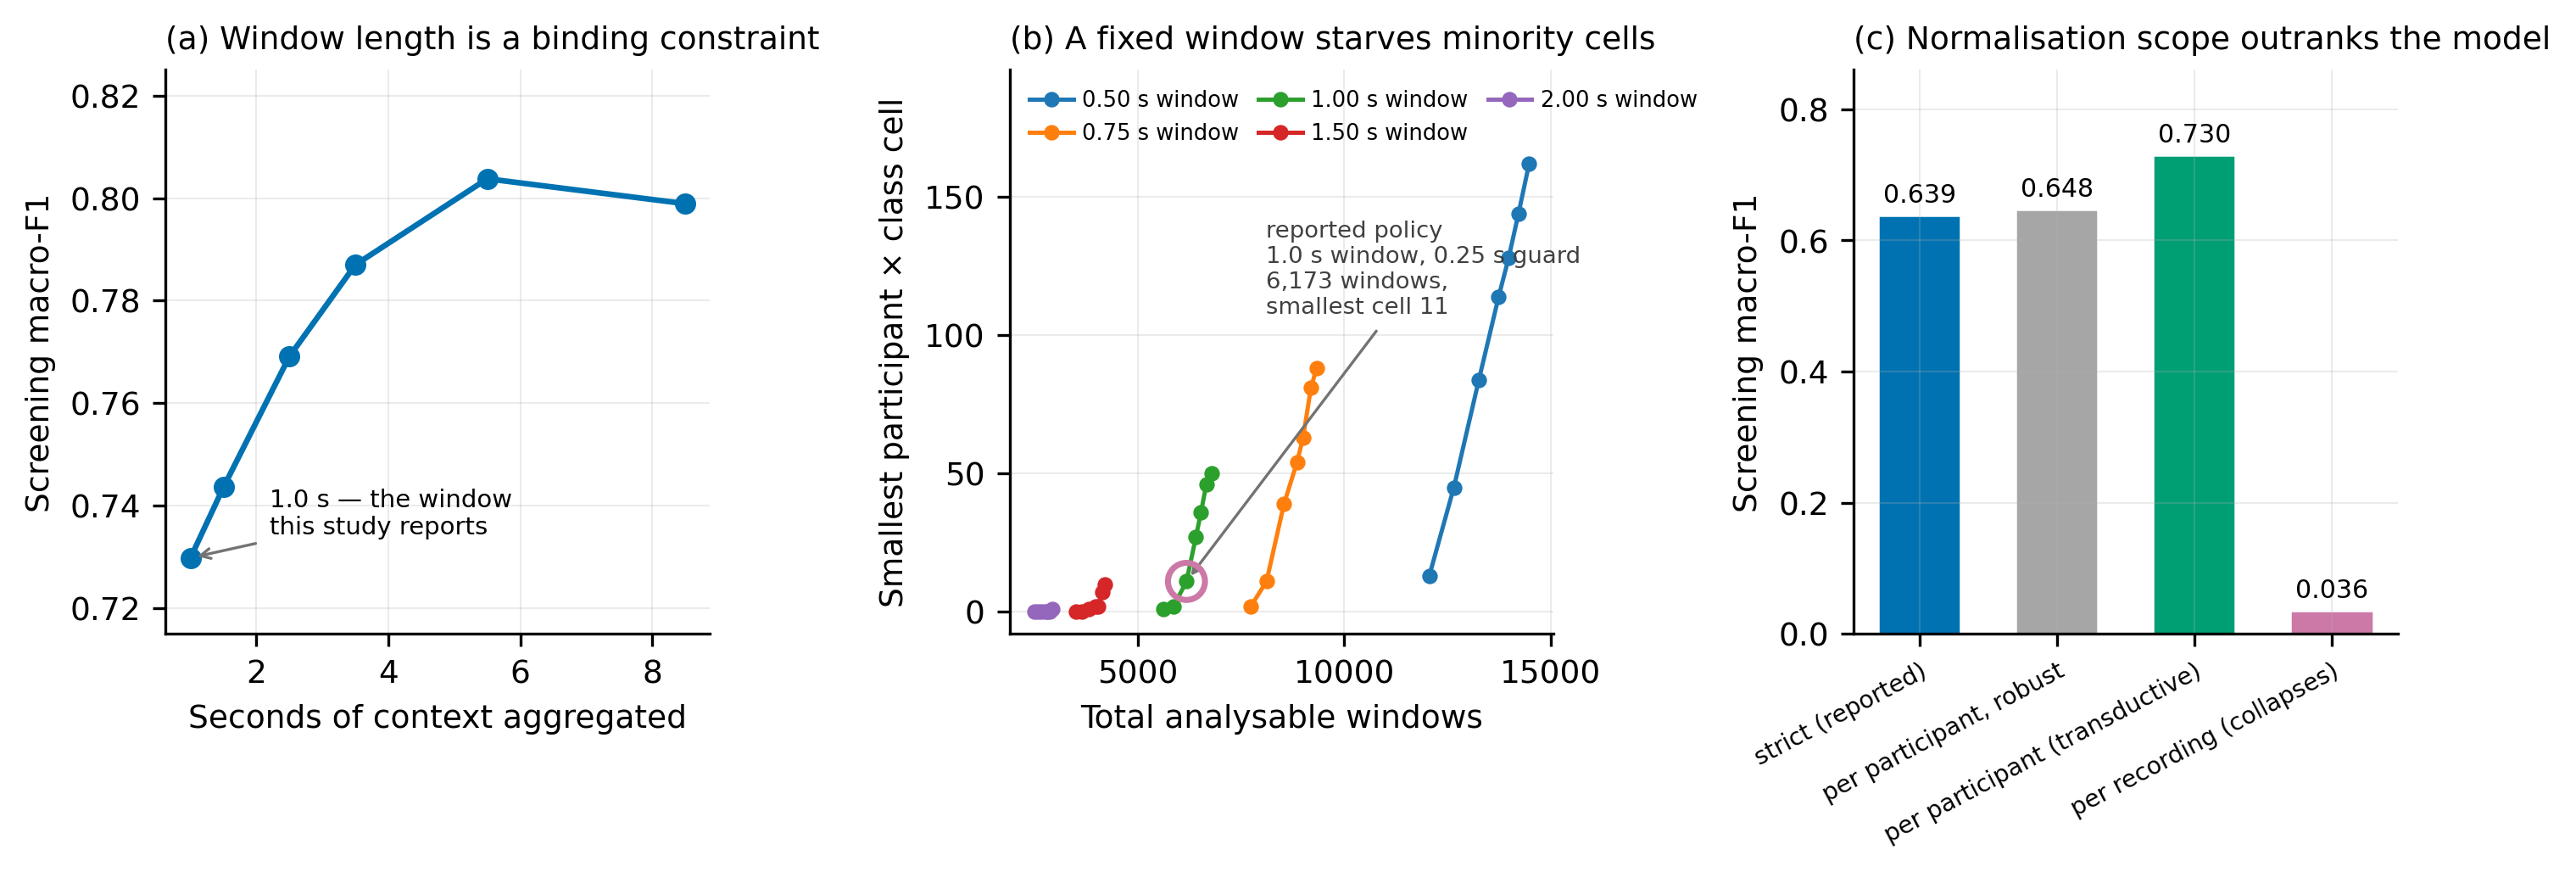
\includegraphics[width=0.98\textwidth]{Figures/v5/design_constraints.png}
  \caption{Three design constraints, measured on identical windows and folds with the screening harness. (a) Macro-F1 against seconds of temporal context aggregated within a recording. (b) Every window and guard setting swept: total analysable windows against the smallest participant-and-class cell, reported policy circled. (c) Normalisation scope; the per-participant scope is used by no reported number.}
  \label{fig:design}
\end{figure*}

\subsection{What Determines Performance}
\label{sec:budget}

Table~\ref{tab:budget} collects the six choices on one scale; the ordering is the paper's main result. Signal quality sets a ceiling that nothing above it can raise: through the superseded chain the best model scored 43.5\% macro-F1, below the 61.3\% the weakest baseline reaches on the corrected signal. The entries are not additive (Table~\ref{tab:budget}, note $^{e}$), three are screening measurements, optimistic in level, and the magnitudes belong to this cohort; what generalises is the ordering.

\begin{table*}[!t]
  \centering
  \caption{What determines performance: six choices priced on the same 6,173 windows and five outer folds, in participant-level macro-F1. Entries are not additive and not all from the same harness (Section~\ref{sec:budget}). ``Reported'' states whether the more favourable setting is the one used in this paper.}
  \label{tab:budget}
  \footnotesize
  \begin{tabular*}{\textwidth}{@{\extracolsep{\fill}}lllrl@{}}
    \toprule
    Choice & Change measured & Harness & $\Delta$ macro-F1 & Reported \\
    \midrule
    Signal quality & 60-Hz notch $\rightarrow$ harmonic notch bank & Confirmatory$^{a}$ & $+29.3$ & Yes \\
    Normalisation scope & Strict $\rightarrow$ per-participant & Screening$^{b}$ & $+9.1$ & No$^{c}$ \\
    Learned representation & Band energies $\rightarrow$ wavelet CNN & Conf./screen.$^{d}$ & $+8.1$ & Yes \\
    Temporal context & 1.0 s $\rightarrow$ 5.5 s within a trial & Screening$^{b,e}$ & $+7.4$ & No$^{e}$ \\
    Rhythm representation & Compact $\rightarrow$ extended wavelet CNN & Arch.\ sweep & $+2.8$ & Secondary \\
    Capacity, raw signal & Wavelet CNN $\rightarrow$ early-fusion ($3.2\times$) & Arch.\ sweep & $-3.3$ & No \\
    \bottomrule
  \end{tabular*}
  \begin{flushleft}\footnotesize
  $^{a}$Nested LOSO, three seeds, both arms the EMG-plus-microphone condition (Table~\ref{tab:filter}). $^{b}$Screening harness: optimistic in level, reliable in direction. $^{c}$Legitimate, but presumes a per-user fitting session. $^{d}$Confirmatory network against a screening baseline, the conservative direction. $^{e}$Trial-level: every recording holds one condition. Its 1.0-s baseline is the per-participant scope of the second row, so the two rows share a baseline and must not be summed.
  \end{flushleft}
\end{table*}

\section{Discussion}

\subsection{What the Ordering Means}

What a model could represent mattered more than how large it was, and signal quality set the ceiling for both. Within the wavelet pair, the model that could also represent rhythm beat the one that could not, which converges with RQ4: the rhythm the extended model represents is the information the 1.0-s window withholds, worth 7.4 points against the architecture's 2.8. The binding limitation is informational rather than architectural: a longer window would likely gain more than a larger model. RQ1 is easy to overstate: mains correction is not generally worth 29.3 points, and with clean recordings it is worth nothing; the claim is that the ceiling exists, that its height is measurable, and that nothing above it can be interpreted until it has been measured.

\subsection{Why Signal Validation Belongs Inside the Pipeline}

The defect did not look like a signal problem. It looked like between-participant heterogeneity, the failure mode that motivates transfer learning and larger cohorts, because interference amplitude varies with electrode impedance, cable routing and session rather than with physiology~\cite{deluca2010filtering,besomi2019consensus}, LOSO attributes that variation to the person held out, and the result is the distribution shift that domain generalisation sets out to absorb~\cite{wang2022generalizing}. The code implemented the recommended filter~\cite{chowdhury2013surface,raez2006techniques}; what was missing was one comparison, the response drawn over the measured spectrum of the recordings, and one statistic, the share of in-band power near each mains multiple. That is the argument for making validation a stage of the pipeline that can refuse.

\subsection{What Transfers Beyond This Case Study}
\label{sec:transfer}

Nothing in the procedure is specific to EMG or to bruxism. Nor is it an ablation study, which varies parts of a model; the budget varies the stages upstream of the model, on identical windows and folds. Audit the signal against what the analysis assumes and publish the resulting statistics beside the accuracy; fix the windows, folds and labels and vary one stage at a time; include the choices made before any model was trained; report a budget beside the accuracy, naming each row's harness and baseline; and keep a prediction ledger from which every number is regenerated. EEG, where preprocessing choices are contested~\cite{delorme2023eeg} and architectures are compared under one unpriced pipeline~\cite{bouthillier2021accounting}, is the obvious next case. What does not transfer is the numbers: clean mains would make the first row of Table~\ref{tab:budget} worth nothing, a modality without rhythmic content would make temporal context worth less, and balanced classes would make normalisation scope worth less.

\subsection{Limitations and Next Steps}

The principal limitation is the cohort size, $N=5$: 6,173 overlapping windows do not replace independent participants, one of whom contributed 27\% of them, and LOSO does not establish external generalisation from five people~\cite{varoquaux2018cross}. The budget is an ordering with approximate magnitudes, not a decomposition of variance, and the RQ1 contrast, although conservative in protocol, compares runs from two codebase versions on verified byte-identical windows. The classes are instructed laboratory conditions, not the consensus definition of bruxism~\cite{lobbezoo2018international}: the tasks omit bracing and thrusting~\cite{verhoeff2025definitions}, the diagnoses were not phenotyped~\cite{manfredini2024standardised}, labels rest on a button press, instructed activity may be more regular than spontaneous activity~\cite{farella2008masticatory}, and rest did not sample speaking, swallowing or head movement, so the analysis estimates confusion against quiet rest, not false alarms per hour; pooled-validation accuracies above 90\%~\cite{sonmezocak2021detection} are not like-for-like. Chewing carries the headline accuracy, and part of the clenching-and-grinding confusion is label ambiguity, since a grinding bout's static phases may legitimately carry either label~\cite{lan2022comparative}. A next study should aggregate over a declared temporal context, standardise trigger use, and record over several days with a defined background class; nothing about sleep follows from these awake tasks~\cite{lavigne1996sleep,casett2017validity}.

\section{Conclusion}

This study asked which stages of one biosignal classification pipeline account for its performance, and answered by measurement. On unseen participants the pipeline separated quiet rest and four instructed jaw activities at 81.7\% accuracy and 72.0\% macro-F1 with 5,901 parameters. The ordering is the more durable result: signal quality set a ceiling, a mains-harmonic defect the conventional chain had left untouched being worth 29.3 points of macro-F1; above it, what a model could represent mattered more than its size; and two choices fixed before any model was trained, temporal context and normalisation scope, were each worth as much as the architecture or more. The transferable recommendation costs one pass over the data: report a measured interference statistic beside every accuracy, draw filter responses over the measured spectrum, and fingerprint every channel of every recording. This study does not validate a bruxism detection device; it shows that surface EMG with a wavelet representation merits a larger, phenotyped, multi-day evaluation, and that between any recording and a reported accuracy sit half a dozen stages, each of which can be worth more than the model and each of which can be priced with the data already in hand.

\section*{Supplementary Materials}

The Supplementary Materials contain the positioning comparison with prior studies (Table~S-I); the dataset, guard and training configuration (Table~S-II); the secondary analyses (Table~S-III); the preprocessing chain on a real excerpt (Fig.~S1); the RQ1 mechanism in signal terms (Fig.~S2); per-class ROC curves and a t-SNE of the learned representation (Fig.~S3); signal excerpts with the 1.0-s window drawn to scale (Fig.~S4); training curves (Fig.~S5); and the data, code and artifact-provenance statements.

\section*{Acknowledgment}

The authors thank University of Rhode Island students Anjolaoluwa Akingbile, Jessica Constantine and Nathan DeSalvo, who located and summarised the functions of bruxism devices before this project. The authors declare no competing interests.

\IEEEtriggeratref{40}
\bibliographystyle{IEEEtran}
\bibliography{refs_v8}

\end{document}
